\documentclass[11pt, a4paper]{article}
\usepackage[paper=a4paper, left=1.5cm, right=1.5cm, bottom=1.5cm, top=1.5cm]{geometry}

\usepackage[utf8]{inputenc}
\usepackage[T1]{fontenc}
\usepackage[spanish]{babel}
\usepackage[section]{placeins}
\usepackage{caratula/caratula}
\usepackage{listings}
\usepackage{algpseudocode}
\usepackage{graphicx}
\usepackage{float}
\usepackage{amsmath}
%\usepackage{adjustbox}
\usepackage{blindtext}
\usepackage{sidecap}
\usepackage{color}
\usepackage{subfigure}

\usepackage{xspace}
\usepackage{xargs} %Para crear funciones con muchos argumentos
\usepackage{ifthen}
\usepackage{algorithm}% http://ctan.org/pkg/algorithms
%\usepackage{algorithmic} %paquete para hacer pseudocodigo
\usepackage{titlesec}%http://foro-c.com/blog/latex-formato-de-titulos-de-capitulos-secciones-etc/
\usepackage{setspace}
\usepackage{fancyhdr}
\usepackage[colorlinks=true, linkcolor=blue]{hyperref} %Links para el indice.
\usepackage{float} %Insercion de imagenes flotantes
\usepackage{ stmaryrd }
 	
\usepackage{caption}
\usepackage{subcaption}

\begin{document}

\titulo{Trabajo Práctico \#2}
\fecha{8 de Diciembre de 2013}
\materia{Sistemas operativos}
% \grupo{Grupo Faisán}
\integrante{Leandro Matayoshi}{79/11}{leandro.matayoshi@gmail.com}
\integrante{Martin Santos}{413/11}{martin.n.santos@gmail.com}
\integrante{Alexander Szyrej}{642/11}{luzbelito.as@gmail.com}

%Carátula
\maketitle
\newpage
%Indice
\tableofcontents
\newpage


\section{Introducción}
MongoDB es una base de datos cross-platform orientada a documentos, clasificada como NoSQL y que implementa el paradigma MapReduce para análisis de datos.


El objetivo de este trabajo consiste en comprender e implementar distintos algoritmos de análisis de datos sobre una peque\~na base de datos de $Rededit$ y efectuar un análisis de escalabilidad y performance de la arquitectura utilizando MongoDB para el soporte de los datos y una arquitectura basada en maquinas virtuales.


Para esto último se consideran distintas alternativas de $HaaS$ (Hardware as a Service) para hacer el despliegue de las máquinas virtuales, evaluando performance considerando las capacidades de MongoDB.


\section{Desarrollo}
Debemos realizar un manejo eficiente de la base de datos de \emph{Rededit}. Analicemos la estructura del razonamiento que 
nos lleva a usar \emph{Haas} como una de las mejores alternativas para cumplir con este objetivo:

~

\begin{figure}[!h]
	\begin{center}
		  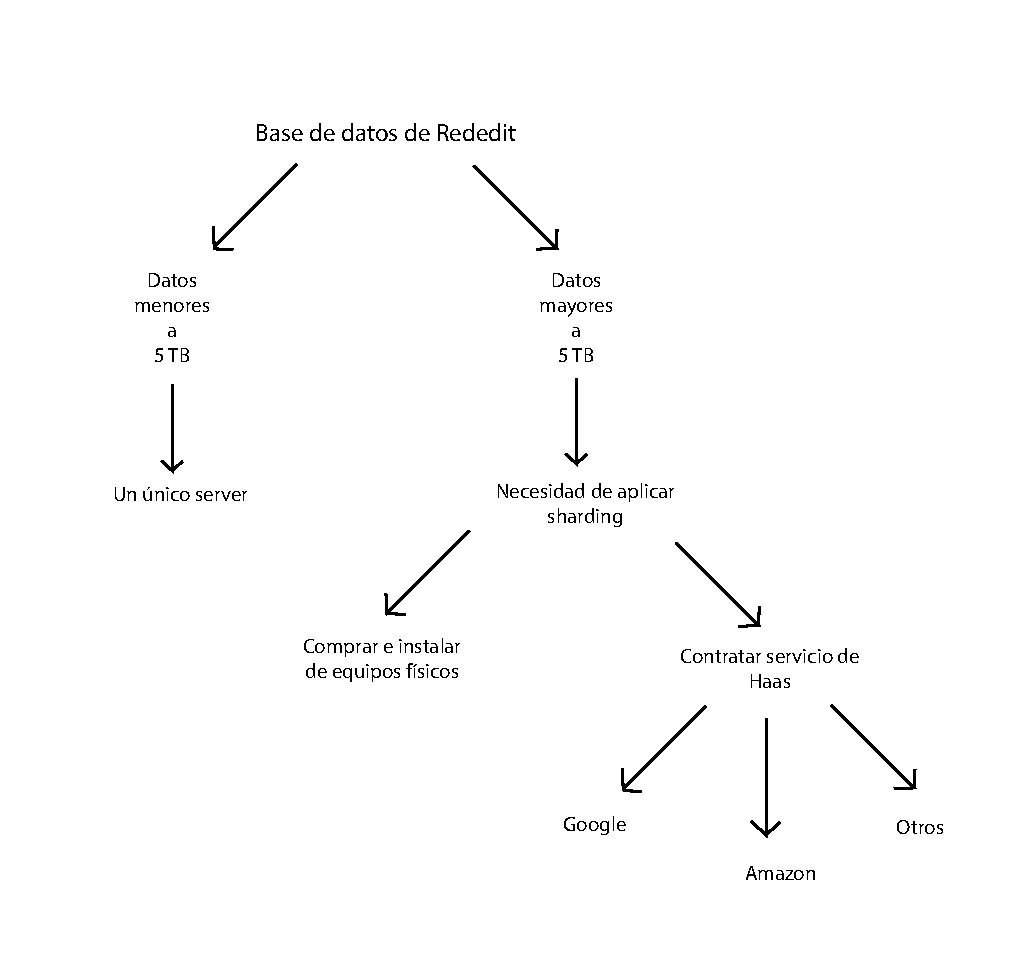
\includegraphics[keepaspectratio]{imagenes/im_1.pdf}
		  \caption{Cada nuevo par de juntas introduce 4 nuevas fuerzas}
		  \label{fig:contra1}
	\end{center}
\end{figure}
\FloatBarrier

\subsection{Una única instancia de MongoDB. Prueba de concepto MapReduce}


En esta sección implementaremos distintos algoritmos de análisis de datos para operar sobre una peque\~na colección de posts de $Rededit$, con un tama\~no aproximado de 17MB. Dado el peque\~no volumen de datos con el cual trabajaremos dispondremos de una única instancia de MongoDB (no sharding).


Queremos:
\begin{itemize}
	\item Analizar la reacción de la comunidad en promedio frente a posts de otros usuarios.
	\item Calcular un promedio de comentarios por submission.
	\item Encontrar el usuario con mayor score.
	\item Determinar en que horario se producen más comentarios, y en cual se comenta menos.
\end{itemize}


\subsubsection{Comunidad Upvoter-Neutral-Downvoter}

Queremos analizar el comportamiento de la comunidad en base a una reducida colección de posts. Para determinar el vote-trend implementamos un único MapReduce sobre la colección de posts.


La función \textbf{map} genera $cuatro$ claves:
\begin{itemize}
	\item $posts-upvoted$ obtiene un nuevo valor '1' por cada post donde los comentarios positivos superan en cantidad a los negativos.
	\item $posts-downvoted$, a la inversa que el anterior, obtiene un nuevo valor '1' por cada post donde los downvotes superan a los upvotes.
	\item $neutral-posts$ recibe un valor '1' por cada post donde los downvotes igualan en cantidad a los upvotes.
	\item $vote-trend$ recibe un '1' por cada $post-upvoted$ y un '-1' por cada $post-downvoted$.
\end{itemize}


La función \textbf{reduce} se reduce en sumar todos los valores para cada clave. De esta forma contabilizamos los posts de votos positivos, los negativos y los neutrales, y al mismo tiempo calculamos el $vote-trend$ de manera tal que si el resultado es positivo la comunidad podría definirse como $upvoter$, $downvoter$ de lo contrario o $neutral$ si $vote-trend$ es exactamente cero.

~

Con 21270 $downvoted-posts$, 106092 $upvoted-posts$ y 4941 $neutral-posts$, el $vote-trend$ da como resultado 84821, lo cual indica que la comunidad es upvoter.

\subsubsection{Comentarios por submission}

Queremos encontrar en promedio cuantos comentarios se realizan por cada submission. Para ello se implementa un único MapReduce sobre la colección de posts en conjunto con la función finalize para calcular el promedio final.

~

La función \textbf{map} genera una única clave $comments$ donde por cada post se genera un valor compuesto por el número de comentarios del mismo y un field $count$ para contabilizar la cantidad de posts.


La función \textbf{reduce} hace la suma total de todos los comentarios y los posts (count).


Luego de que se efectuan los reduce necesarios, se procede con la función \textbf{finalize}, la cual calcula el promedio de comentarios teniendo ya el número total de comentarios (sum($comments$)) y el número de posts (sum($count$)).

~

Como resultado obtuvimos que, en promedio, se efectuan alrededor de 39 comentarios por submission.

\subsubsection{Usuario con más puntaje}

Queremos encontrar el usuario cuya suma de los scores de sus posts supere la de los demás. Para ello encadenamos dos MapReduce: el primero sobre la colección posts y el segundo sobre la colección generada por el primer MapReduce.

~

El primer MapReduce se resume en generar una clave por cada usuario, cada una emitida conjuntamente con su score. Luego se suman todos los scores para cada usuario y de esa manera se obtiene el score total de cada uno.

El segundo MapReduce consiste en encontrar, dados los scores totales de cada uno de los usuarios, aquel que suma más que el resto. Para ello se emite una única clave 'max', con valores asociados compuestos por una tupla usuario-score por cada usuario de nuestra red. Luego durante el reduce tomamos el usuario con el máximo score dentro de nuestra lista de values. 

~

Encontramos que el usuario con mayor score es 'nombre vacio' con 1311814 pts.

\subsubsection{Horario más y menos activo}

Queremos encontrar el horario en el cual la comunidad participa más comentando posts, es decir, determinar de alguna manera el mejor horario para postear. Análogamente determinamos el horario en el cual menos se comenta. Para ello utilizamos nuevamente dos MapReduce encadenados.

~

El primer MapReduce se resume en generar una clave por hora, es decir un total de 24 claves. Para ello se utiliza la función $substring(int idx0, int idxn)$ para quedarnos a partir del $raw-time$ sólo con la hora en la cual fue subido el post. Cada una de ellas viene acompa\~nada por un valor igual al número de comentarios de dicho post. El reduce sólo calcula la suma de todos los comentarios en una determinada hora.

El segundo MapReduce, semejante al punto anterior, consiste en encontrar la hora cuyo número de comentarios es máximo, y aquella que minimiza dicho valor.

~

Encontramos que los posts subidos de 00:00 a 01:00 son aquellos que más comentarios suman, con un total de 632402 comentarios. Luego de 01:00 a 02:00 es el horario en el cual menos comentarios hay, con tan solo 91634, lo cual parece ser razonable si pensamos que el momento pico de actividad es antes de ir a dormir.


\subsection{Sharding, conceptos generales}

''Sharding is the process of storing data records across multiple machines and is MongoDB’s approach to meeting the
demands of data growth. As the size of the data increases, a single machine may not be sufficient to store the data nor
provide an acceptable read and write throughput. Sharding solves the problem with horizontal scaling. With sharding,
you add more machines to support data growth and the demands of read and write operations.'' (MongoDB-sharding-guide)

''Vertical scaling adds more CPU and storage resources to increase capacity. Scaling by adding capacity has lim-
itations: high performance systems with large numbers of CPUs and large amount of RAM are disproportionately
more expensive than smaller systems. Additionally, cloud-based providers may only allow users to provision smaller
instances. As a result there is a practical maximum capability for vertical scaling.'' (MongoDB-sharding-guide)

''Sharding, or horizontal scaling, by contrast, divides the data set and distributes the data over multiple servers, or
shards. Each shard is an independent database, and collectively, the shards make up a single logical database.''

\subsection{Sharding en MongoDB}

MongoDB soporta sharding a través de estructuras llamadas \emph{sharded clusters},
que cuentan con los siguientes componentes:

\begin{itemize}
	\item Shards o \emph{mongods}
	\item Query routers o \emph{mongos}
	\item Config servers 
\end{itemize}

Shards o \emph{mongods} son los nodos de almacenamiento de datos. Cada nodo está compuesto por un \emph{replica sets}. 
Los Query routers o \emph{mongos} actúan de intermediarios entre los pedidos de los clientes y los shards correspondientes
que contienen esos datos específicos. Un cluster puede contener más de un query router (y es conveniente que así) sea,
para disminuír cantidad de pedidos que debe manejar un único nodo.
Finalmente, los Config servers almacenan la metadata del cluster: principalmente, el mapeo de los datos en cada uno de los
shards.

\subsection{Decisiones de arquitectura}

Para establecer la base de datos de \emph{Rededit} tomamos las siguientes decisiones de arquitectura:

\subsubsection{\emph{Mongods y Replica sets}}

Cada \emph{shard} está constituido por un \emph{replica set}: un conjunto de procesos que mejoran la 
disponibilidad de los datos del
servidor en base a la redundancia. Existen tres tipos de miembros:

\begin{description}
	\item[Primario] Recibe las operaciones de escritura.
	\item[Secundario] Replican las mismas operaciones efectuadas por el primario para mantener el set de datos consistente.
	\item[Árbitro] Opcional. 
	No almacena datos. Simplemente participa en la elección de un nuevo nodo primario en los casos en donde el actual se
	encuentra inhabilitado.
\end{description}

Decidimos adoptar una de las configuraciones típicas que propone \emph{MongoDB-replication-guide}: 
Una estructura conformada por tres nodos, todas ellas almacenando datos: 

\begin{description}
	\item[Uno primario] 
	\item[Dos secundarios] Ambos son candidatos a volverse primarios luego de una elección, en el caso de una falla
	en el nodo primario.
	\item[Ningún árbitro]
\end{description}

Mediante esta elección disponemos de 2 copias completas del set de datos además del primario. Provee tolerancia a fallos
en el nodo primario, y buena velocidad de respuesta debido a la redundancia.

\subsubsection{Config servers}

El cluster va a contar con 3 servidores de configuración (Cantidad sugerida por \emph{MongoDB-sharding-guide}).














\section{Conclusiones}
%Durante el transcurso de este trabajo pr\'actico comprendimos los usos y ventajas del paradigma MapReduce para an\'alisis de datos en sistemas distribuidos, 
as\'i como tambien las ventajas de montar un proyecto sobre HaaS, evaluando distintas alternativas de dicho servicio.
Entendemos que 


\end{document}
